%\documentclass[10pt]{beamer}
\documentclass[10pt,handout]{beamer}
\usepackage[spanish]{babel}
% % \usepackage[backend=biber, style=authoryear-icomp]{biblatex}
\resetcounteronoverlays{exx}
\usepackage{mdframed}
\usepackage{tikz}
\usepackage{blindtext}
\usepackage{tipa}
% \usepackage{cgloss4e}
% \usepackage{gb4e}
% \usepackage{qtree}
\usepackage{cancel}
\usepackage{wrapfig}
\usepackage{soul}
\usepackage{enumerate}
\usepackage{longtable}
\graphicspath{ {./figures/} } % declaramos donde estan las imagenes
\usepackage[labelformat=simple]{subcaption} % para varias imagenes juntas
\renewcommand\thesubfigure{(\alph{subfigure})}
\usepackage[utf8]{inputenc}
\usepackage{amsmath}
\usepackage{amsfonts} % simbolos como el I de matriz identidad
\usepackage{bm}
\usepackage{graphicx} % paquete para ver imagenes
\usepackage{setspace}
\usepackage[T1]{fontenc}
\usepackage{parskip}
\usepackage{color}
\usepackage{framed}

\usetheme{Copenhagen}
\definecolor{frenchblue}{rgb}{0.0, 0.45, 0.73} % ESTE!!!!

\setbeamercolor{block body}{bg=frenchblue!50}
\setbeamercolor*{structure}{fg=frenchblue,bg=blue}
\setbeamercolor{normal text}{fg=black}
\setbeamercolor{frametitle}{bg=black}
\setbeamertemplate{frametitle}[default][center]
\setlength{\parskip}{12pt}
\useoutertheme{infolines} % me comia mucho espacio de la otra fgorma
\makeatother
\setbeamertemplate{footline}
{
  \leavevmode%
  \hbox{%
  \begin{beamercolorbox}[wd=.3\paperwidth,ht=2.25ex,dp=1ex,center]{author in head/foot}%
    \usebeamerfont{author in head/foot}\insertshortauthor
  \end{beamercolorbox}%
  \begin{beamercolorbox}[wd=.6\paperwidth,ht=2.25ex,dp=1ex,center]{title in head/foot}%
    \usebeamerfont{title in head/foot}\insertshorttitle
  \end{beamercolorbox}%
  \begin{beamercolorbox}[wd=.1\paperwidth,ht=2.25ex,dp=1ex,center]{date in head/foot}%
    \insertframenumber{} / \inserttotalframenumber\hspace*{1ex}
  \end{beamercolorbox}}%
  \vskip0pt%
}
\makeatletter
\setbeamertemplate{navigation symbols}{}
%\setbeameroption{show notes}
\setbeameroption{hide notes}


\usepackage{hyperref}

\title[Algoritmos y estructuras de datos 2]{Oblivious Data Structures}
\author[Matias Mazzanti]{Matias Mazzanti}


\institute{DC-UBA}
\date{03 de Agosto de 2022}

\titlegraphic{
\includegraphics[,height=2cm,keepaspectratio]{logo.pdf}     }
%\logo{
\includegraphics[height=2.5cm]{logo.pdf}}

\begin{document}

\begin{frame}

\maketitle

\end{frame}

\section{}
\begin{frame}
\frametitle{}
Criptografia: Codificar mensajes y operaciones por motivos de seguridad.

En particular lo aplicamos a la firma digital incremental de documentos.

Al modificar el documento incremento la firma sin necesidad de hacer una firma nueva.


El documento se divide en bloques y a cada uno se le pone una firma digital convencional.
Cada resultado de estos es una hoja del arbol.
Los nodos internos son tageados con una firma digital de sus hijos y un entero contando
la cantidad de hojas del sub arbol, que tiene de raiz a dicho nodo.
Por cada operacion basica, la firma del documento puse actualizada usando los Algoritmos
de los arboles 2-3 y recomputando las firmas de los nodos internos que fueron modificados.
Operaciones en tiempo O(logn).

Problema: No tiene privacidad. Cada actualizacion contiene informacion de las modificaciones realizadas.

Solución: Estructuras de datos indavertidas (Oblivious) $\rightarrow$ Oblivious trees.

\end{frame}
\section{}
\begin{frame}
\frametitle{}
\begin{figure}[h!]
    \centering
    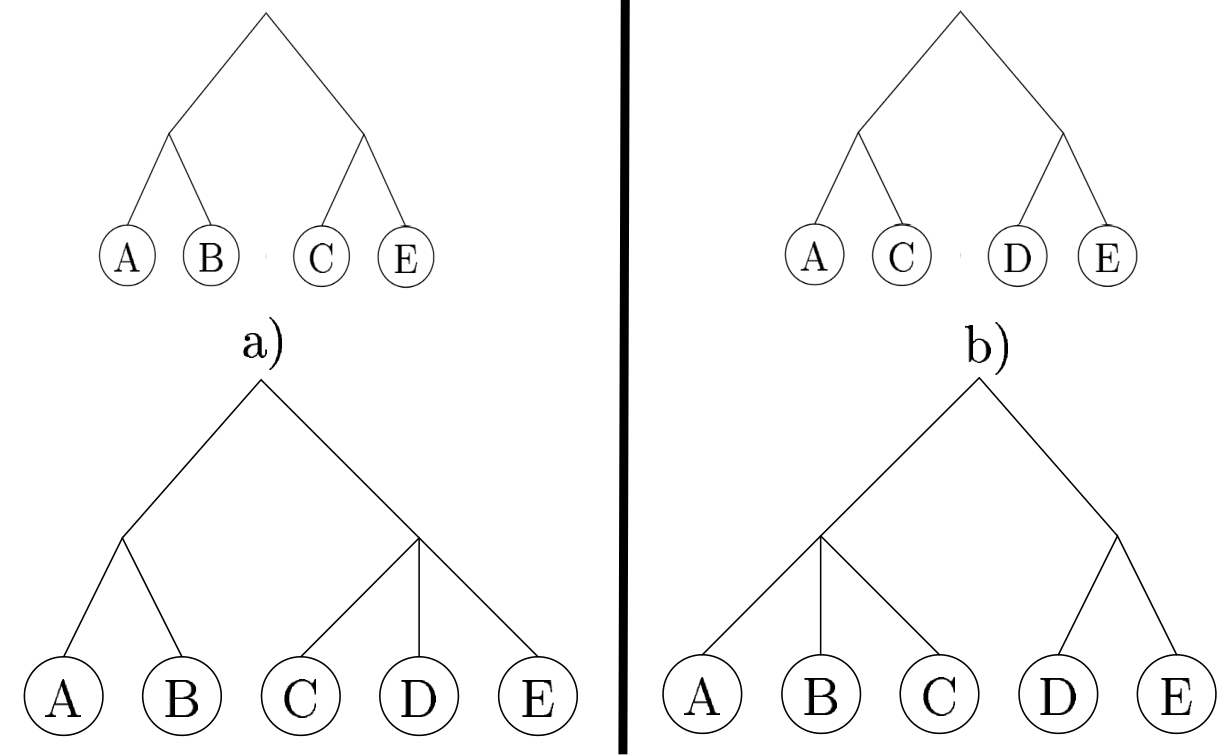
\includegraphics[scale=0.25]{2-3tree.jpg}
\end{figure}


\end{frame}


%%%%%%%%%%%%%%%%%%%%%%%%%%%%%%%%%%%%%%%%%%%%%%%%%%%%%%%%%%%%%%%%%%%%%%%%%%%%%%%%%%%%%%%%%%%%%%%%%%%%
\section{}
\begin{frame}
\frametitle{}
Nos vamos a centrar en arboes
Arboles AVL
Por que lo quiero balanceado.
\end{frame}
%%%%%%%%%%%%%%%%%%%%%%%%%%%%%%%%%%%%%%%%%%%%%%%%%%%%%%%%%%%%%%%%%%%%%%%%%%%%%%%%%%%%%%%%%%%%%%%%%%%%

\section{}
\begin{frame}
\frametitle{}
firma incremental

\end{frame}

%%%%%%%%%%%%%%%%%%%%%%%%%%%%%%%%%%%%%%%%%%%%%%%%%%%%%%%%%%%%%%%%%%%%%%%%%%%%%%%%%%%%%%%%%%%%%%%%%%%%

\section{}
\begin{frame}
\frametitle{}
Por que estos no preservan la privacidad

\end{frame}
%%%%%%%%%%%%%%%%%%%%%%%%%%%%%%%%%%%%%%%%%%%%%%%%%%%%%%%%%%%%%%%%%%%%%%%%%%%%%%%%%%%%%%%%%%%%%%%%%%%%

\section{}
\begin{frame}
\frametitle{B-tree}

\begin{columns}
    \column{0.5\textwidth}
        Arbol autobalanceado de busqueda.

Balanceado: Permite busquedas en peor caso de O(logn).

Busqueda: Mantiene orden dentro del arbol.

Utilizacion: Reducir accesos al disco, (arboles grandes que no entran en memoria principal).

Arboles B de grado M
    \column{0.5\textwidth}
        \begin{itemize}
          \item Cada noto tiene como Maximo M hijos.
          \item Un nodo que no sea hoja con k hijos contiene k-1 claves.
          \item La raiz tiene como minimo 2 hijos a menos que sea hoja.
          \item Todo nodo que no sea ni raiz ni hoja tiene al menos M/2 hijos.
          \item Todas las hojas estan al mismo nivel.
          \item Las claves estan orndeandas en cada nodo.
        \end{itemize}
\end{columns}
\end{frame}
%%%%%%%%%%%%%%%%%%%%%%%%%%%%%%%%%%%%%%%%%%%%%%%%%%%%%%%%%%%%%%%%%%%%%%%%%%%%%%%%%%%%%%%%%%%%%%%%%%%%

\section{}
\begin{frame}
\frametitle{2-3 tree}

Arboles 2-3 es un arbol B de grado 3.
\begin{itemize}
  \item Nodos con 2 hijos (alias 2-nodes) con unica clave.
  \item Nodos con 3 hijos (alias 3-nodes) con dos claves.
\end{itemize}

Insercion: Busco el lugar en orden para la nueva hoja. Si el nodo esta lleno, hago una division.
Ordeno los valores y el del medio sube al nodo padre y los extremos se separan en nuevos nodos.
Se realiza de forma recursiva en caso de necesitarse.
Caso contrario lo agrego en orden.

Borrado: Si el valor esta en un nodo interno: reemplazo el valor que quiero borrar por su
successor en ornden y borro.
Si es una hoja lo borro. Pero si el padre tiene 2 claves y tenia 3 hijos, al quedar con dos se rompe el invariante.
Bajo una de las claves del padre a uno de los nodos.
\end{frame}



%%%%%%%%%%%%%%%%%%%%%%%%%%%%%%%%%%%%%%%%%%%%%%%%%%%%%%%%%%%%%%%%%%%%%%%%%%%%%%%%%%%%%%%%%%%%%%%%%%%%

\section{}
\begin{frame}
\frametitle{Oblivious tree}

Queremos un 2-3 tree pero sin perdida de privacidad.

Modificaciones:
\begin{itemize}
  \item Permite nodos con un unico hijo, solo en caso que sea el ultimo nodo de la derecha.
  \item Toda la información de las firmas esta en las hojas.
  \item Deja de ser una estrucutra deterministica para ser probabilistica.
\end{itemize}

Cada nodo guarda su grado que es la cantidad de hijos que tine.
Tambien guarda su tamaño que es la cantidad de hojas que tiene el subarbol que tiene como
raiz al mismo.
\end{frame}


%%%%%%%%%%%%%%%%%%%%%%%%%%%%%%%%%%%%%%%%%%%%%%%%%%%%%%%%%%%%%%%%%%%%%%%%%%%%%%%%%%%%%%%%%%%%%%%%%%%%

\section{}
\begin{frame}
\frametitle{Estructura de datos inadvertidas}

Definiciones:

Un conjunto S de algoritmos que implementan un cierto conjunto de operaciones sobre el arbol de busqueda es
\texttt{Oblivious} si dada dos secuencias de operaciones $p_i$ y $q_i$ generan un arbol con una secuencias
de valores L y ambos tienen misma distribucion de probabilidad de salida.


Vamos a tener
\begin{itemize}
  \item Crear(L): Construye un nuevo arbol de busqueda con los valores de la secuencia L en las hojas.
  \item Insertar(b,i,T): Inserta una nueva hoja con valor b en la posicion i-esima del arbol T.
  \item Borrar(i,T): Remueve la hoja i-esima del arbol T.
\end{itemize}

Condicion para ser inadvertido.

Insertar(b,i,Crear($L_1$)) tiene la misma distribucion de probabilidad que Crear($L_2$), donde $L_{2}$
se obtiene al insetar en $L_{1}$ el elemento b en la i-esima posicion.

Borrar(i, Crear($L_{1}$)) tiene la misma distribucion de probabilidad que Crear($L_2$), donde $L_{2}$
se obtiene al sacar en $L_{1}$ el elemento en la i-esima posicion.


\end{frame}

%%%%%%%%%%%%%%%%%%%%%%%%%%%%%%%%%%%%%%%%%%%%%%%%%%%%%%%%%%%%%%%%%%%%%%%%%%%%%%%%%%%%%%%%%%%%%%%%%%%%

\section{Algoritmos}
\begin{frame}
\frametitle{Creacion}

  Creacion(L): Crea un nuevo arbol. Bottom-up

  L: Lista de claves.

  Tiempo: O(n)

  Se inicia con todas las claves en las hojas en orden dado.
  Y se arma el arbol de abajo arriba, izquierda a derecha.

\begin{itemize}
  \item Se inicia con la primer clave.
  \item Se obtiene un valor random d={2,3}.
  \item Si en el nivel que estoy tengo esa cantidad de nodos, los hago hijos de
    un nodo padre del nivel superior.
  \item Si no hay esa cantidad, d=cantidad de nodos, y los hago hijos de un nodo
    padre del nivel superior.
  \item Finalizo al no tener mas nodos (raiz).
\end{itemize}

\end{frame}

%%%%%%%%%%%%%%%%%%%%%%%%%%%%%%%%%%%%%%%%%%%%%%%%%%%%%%%%%%%%%%%%%%%%%%%%%%%%%%%%%%%%%%%%%%%%%%%%%%%%

\begin{frame}
\frametitle{Ejemplo creacion}

  \only<1>{\begin{figure}[h!]
    \centering
    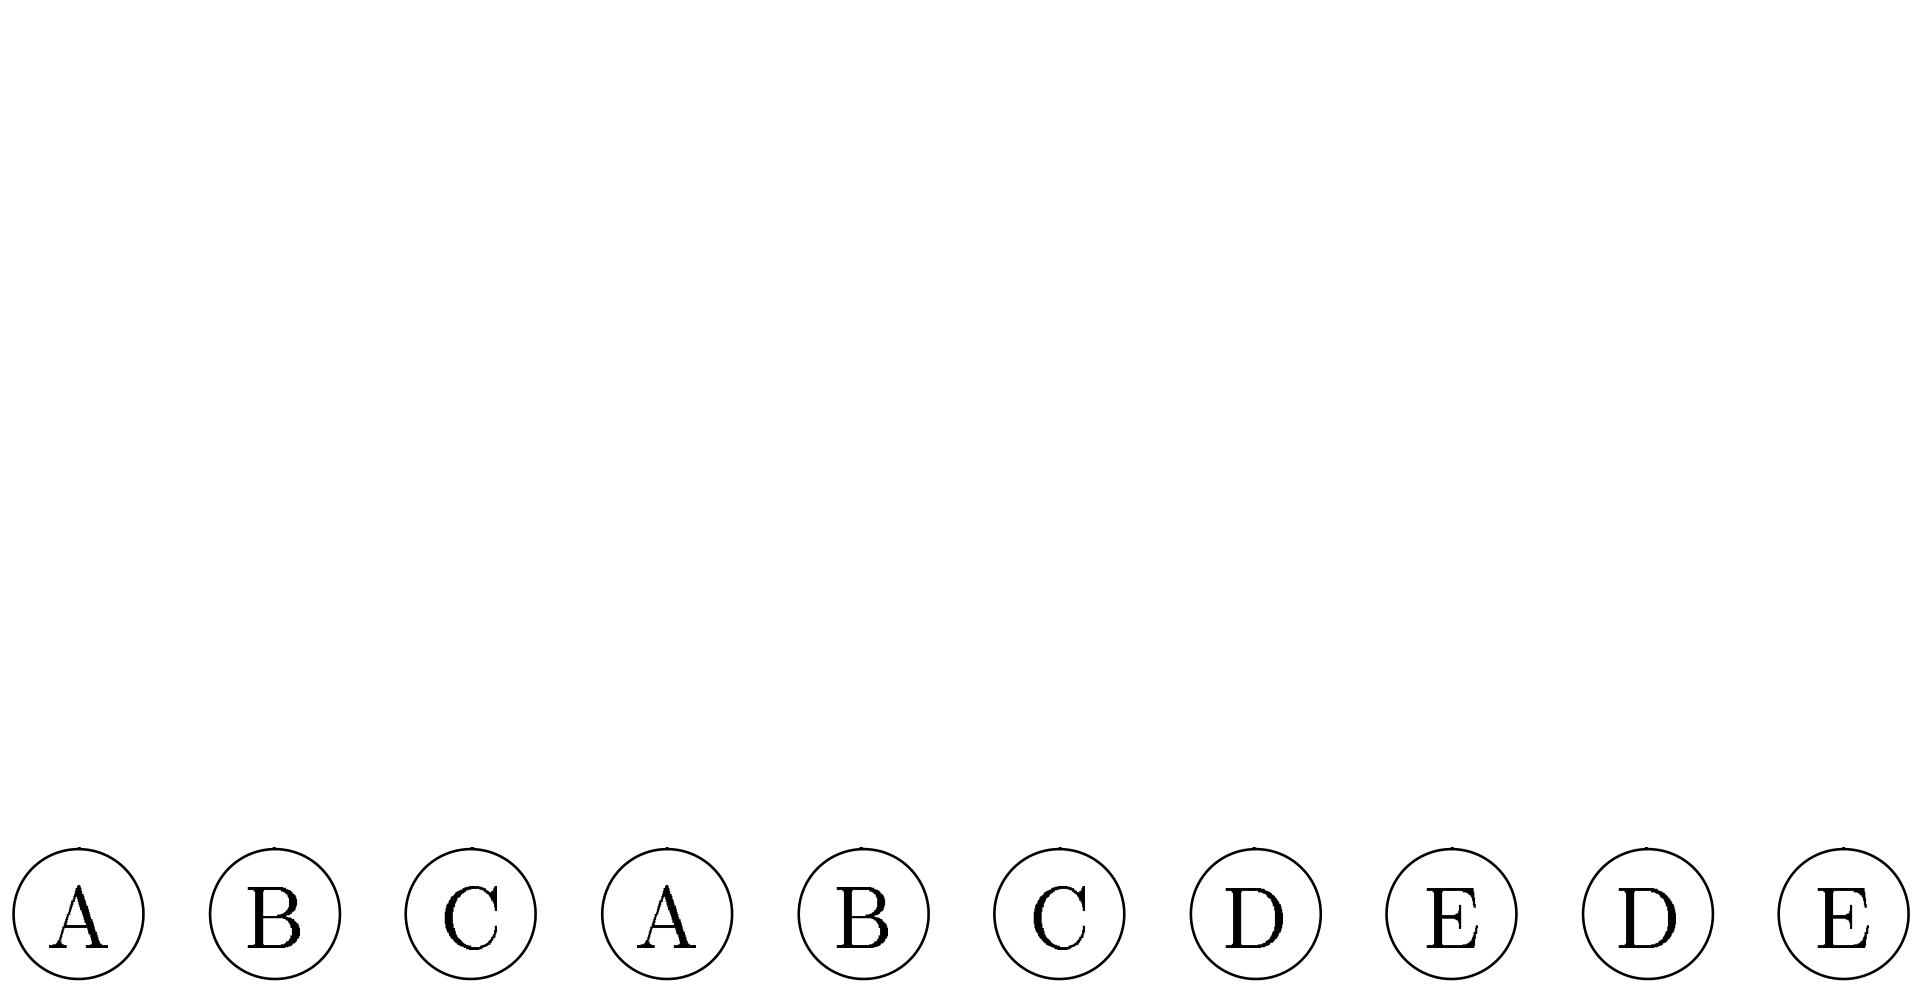
\includegraphics[scale=0.17]{creacionInc.jpg}
\end{figure}}
\pause
  \only<2>{\begin{figure}[h!]
    \centering
    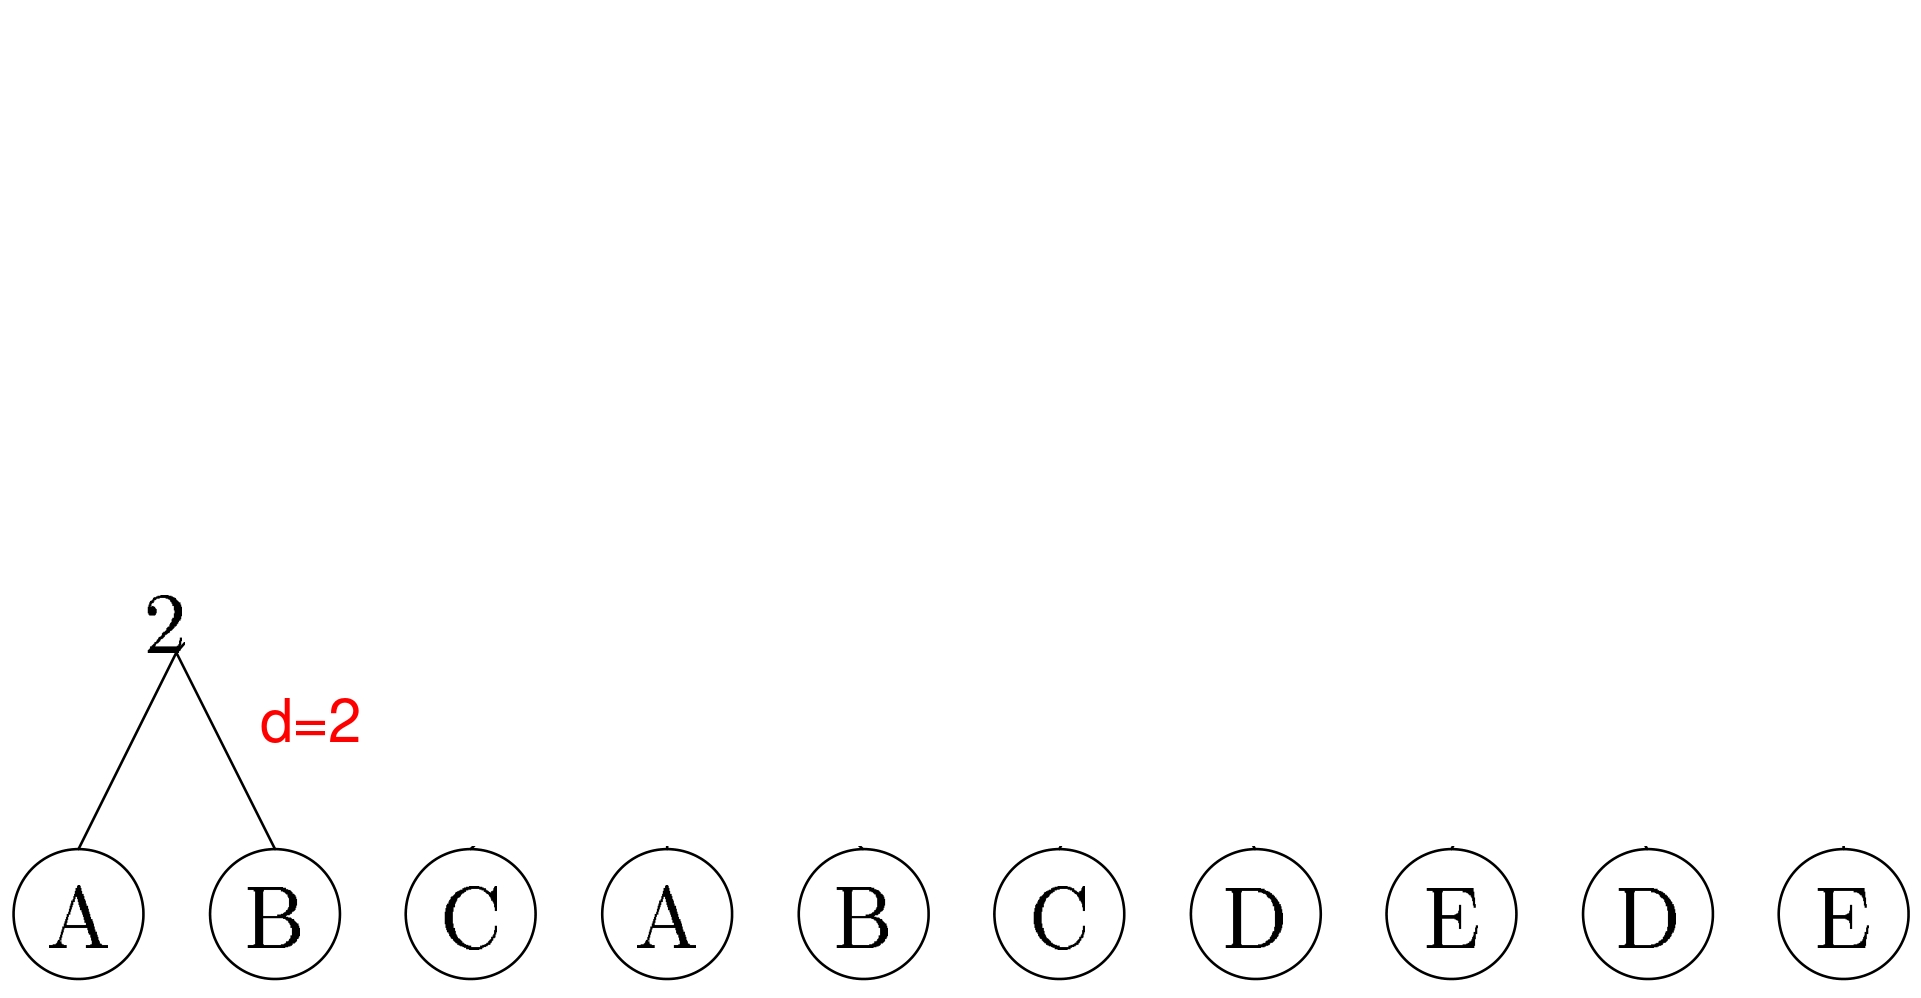
\includegraphics[scale=0.17]{creacion1.jpg}
\end{figure}}
\pause
  \only<3>{\begin{figure}[h!]
    \centering
    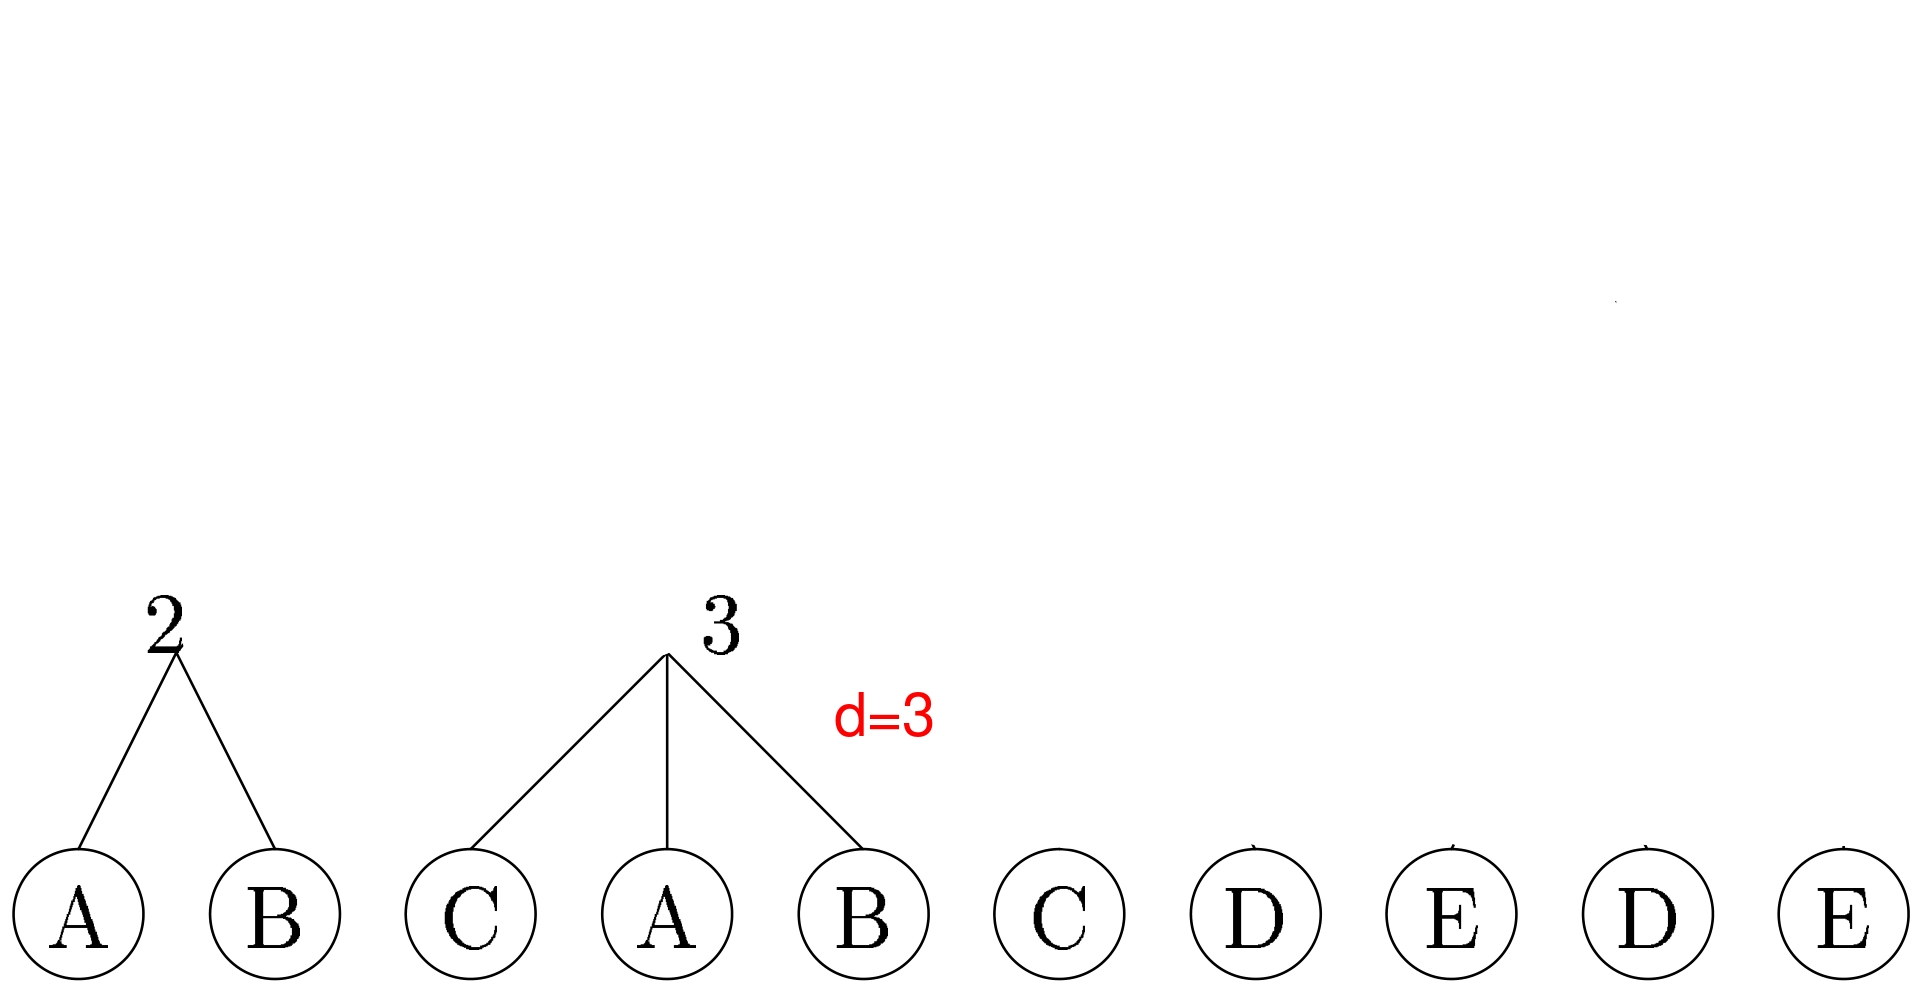
\includegraphics[scale=0.17]{creacion2.jpg}
\end{figure}}
  \pause
  \only<4>{\begin{figure}[h!]
    \centering
    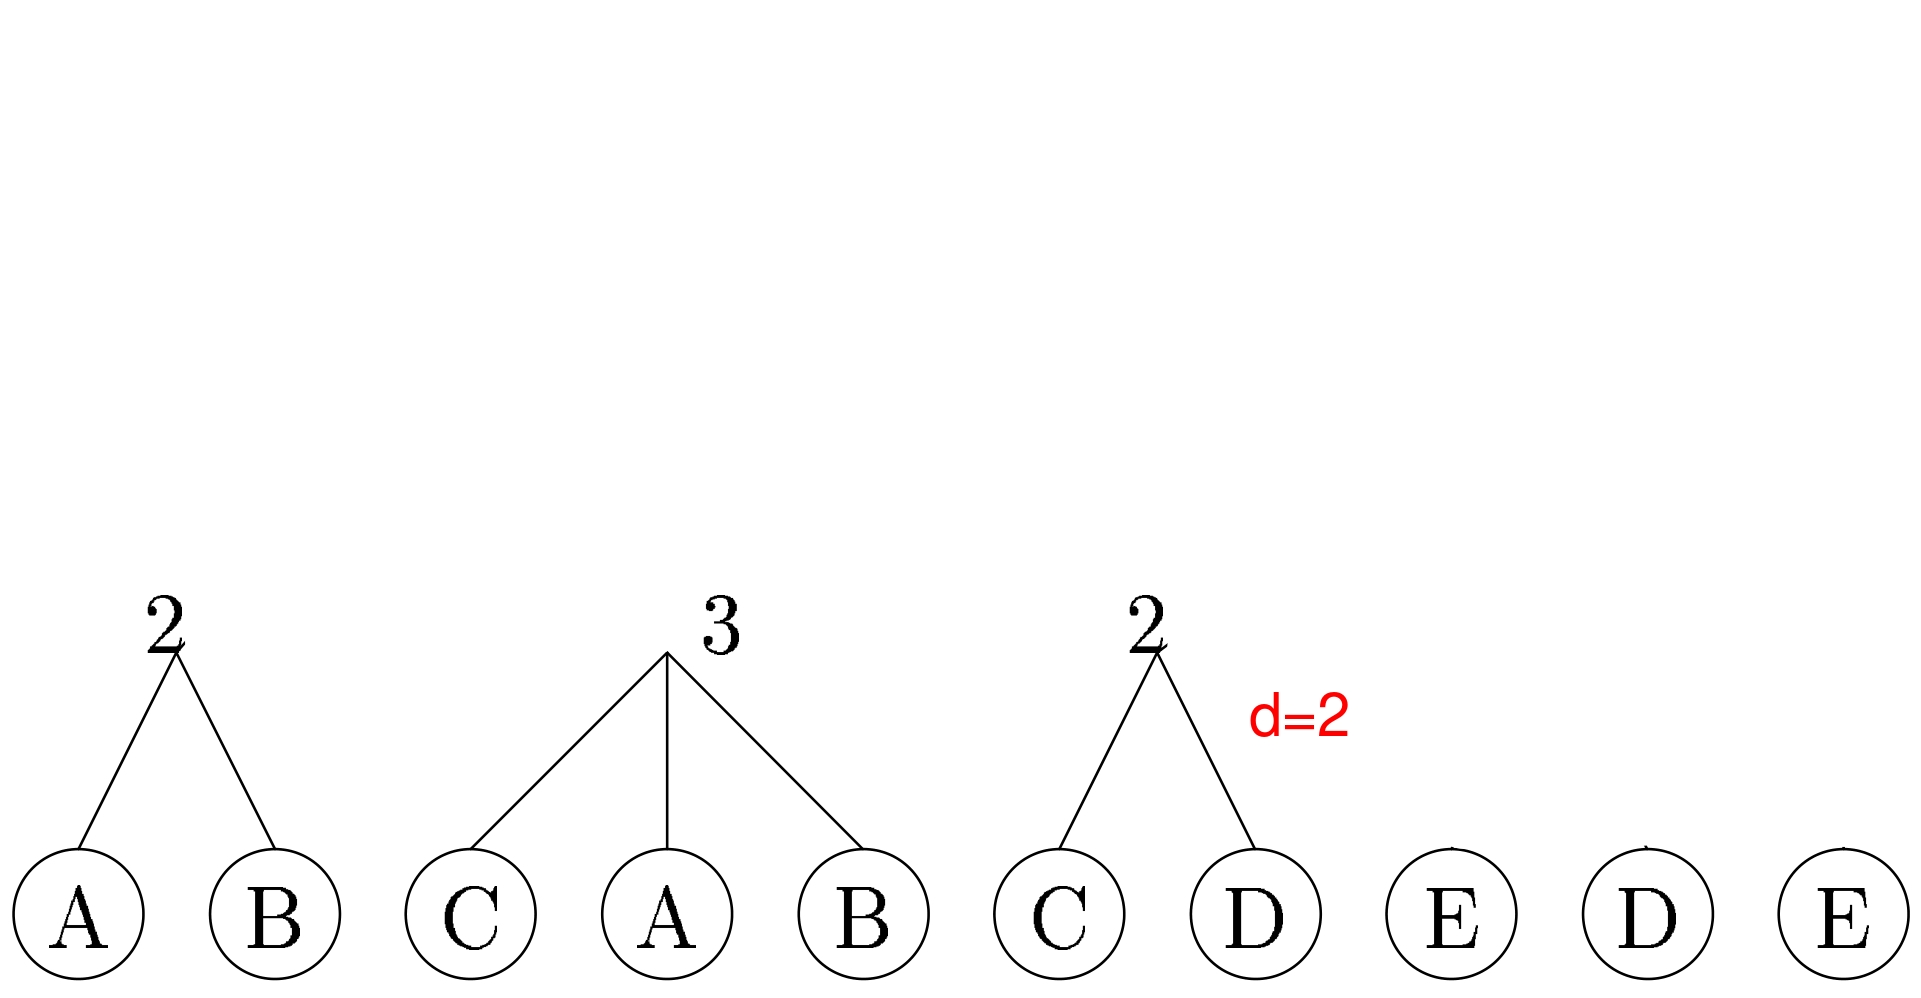
\includegraphics[scale=0.17]{creacion3.jpg}
\end{figure}}
  \pause
  \only<5>{\begin{figure}[h!]
    \centering
    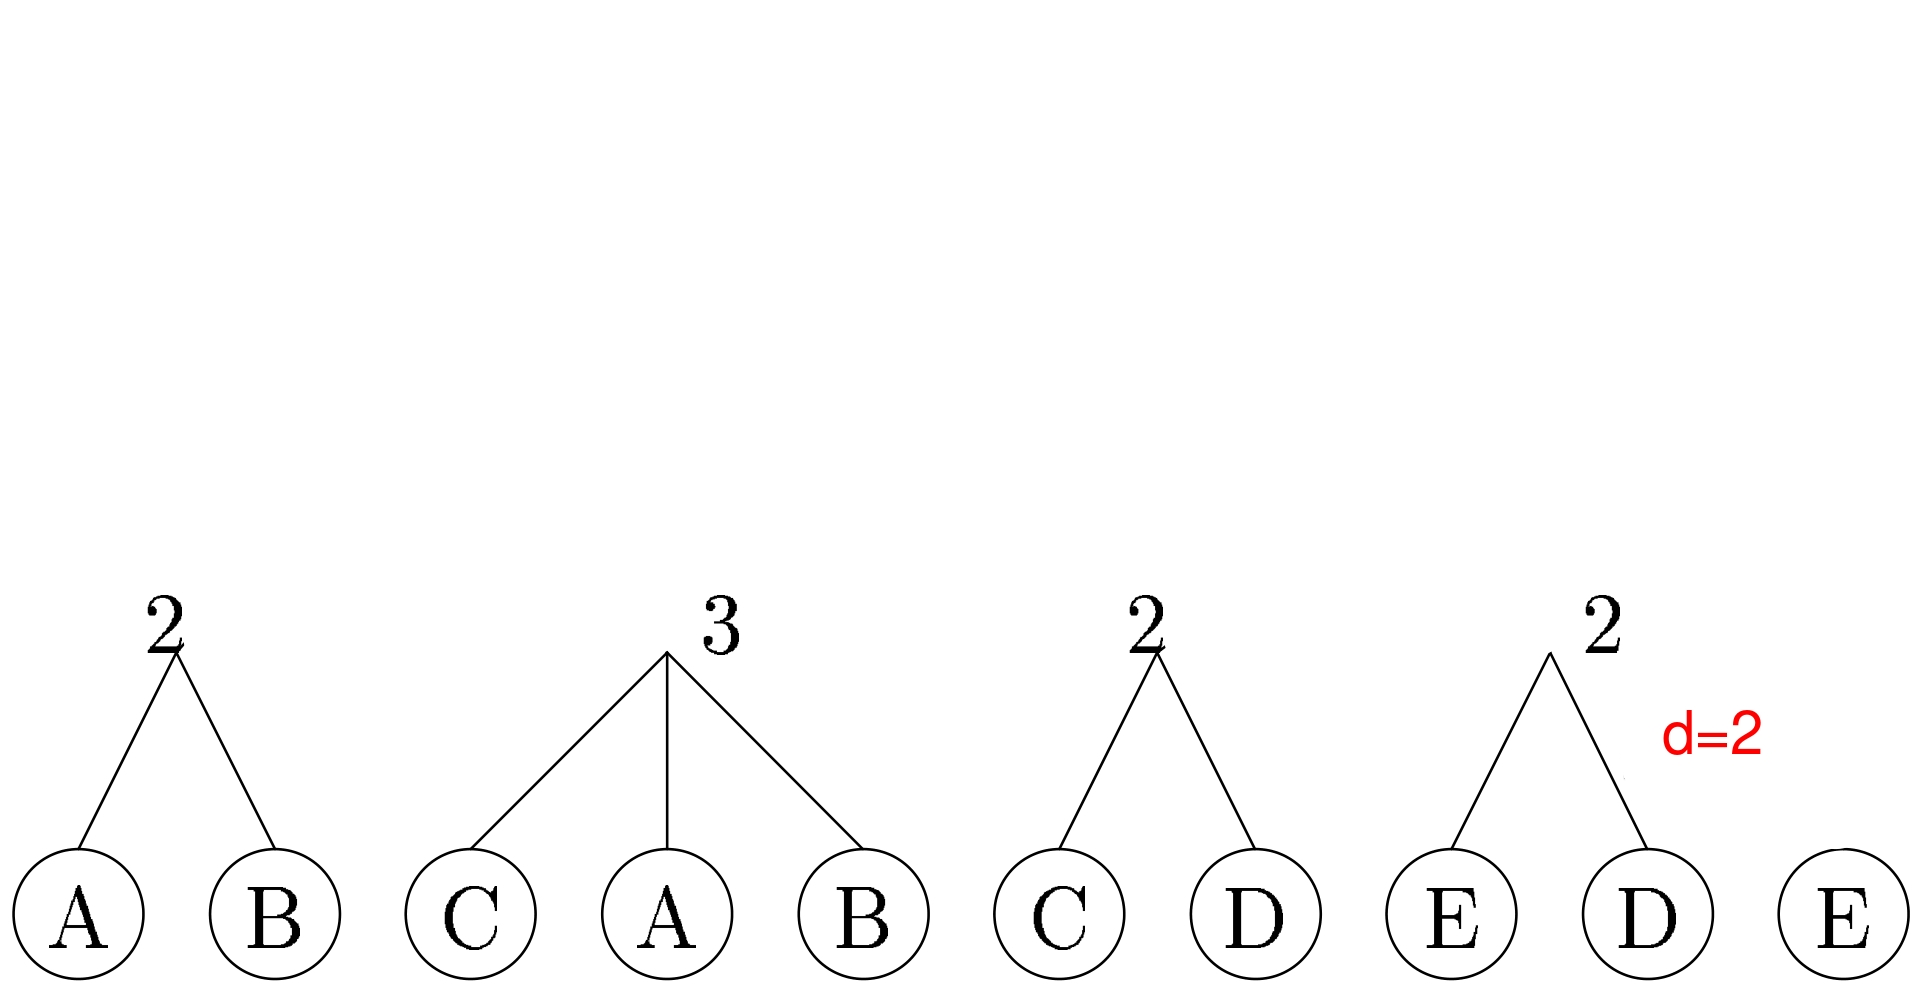
\includegraphics[scale=0.17]{creacion4.jpg}
\end{figure}}
  \pause
  \only<6>{\begin{figure}[h!]
    \centering
    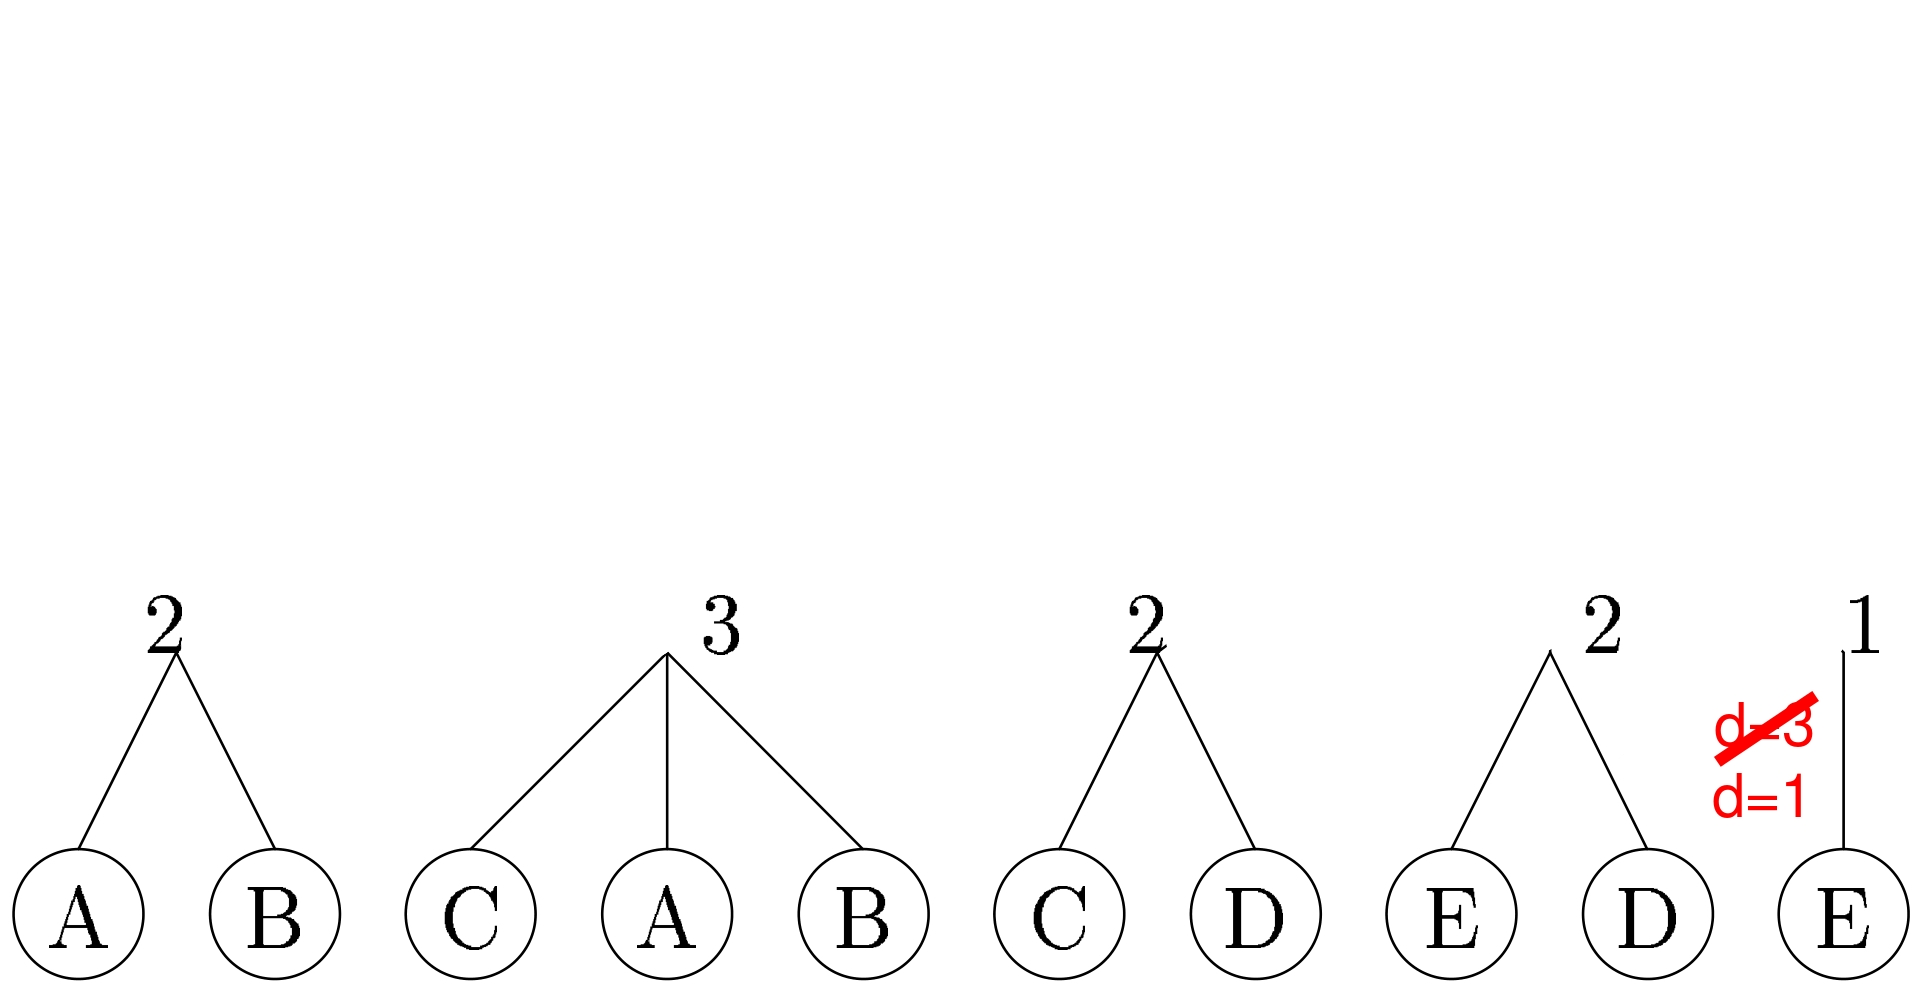
\includegraphics[scale=0.17]{creacion5.jpg}
\end{figure}}
  \pause
  \only<7>{\begin{figure}[h!]
    \centering
    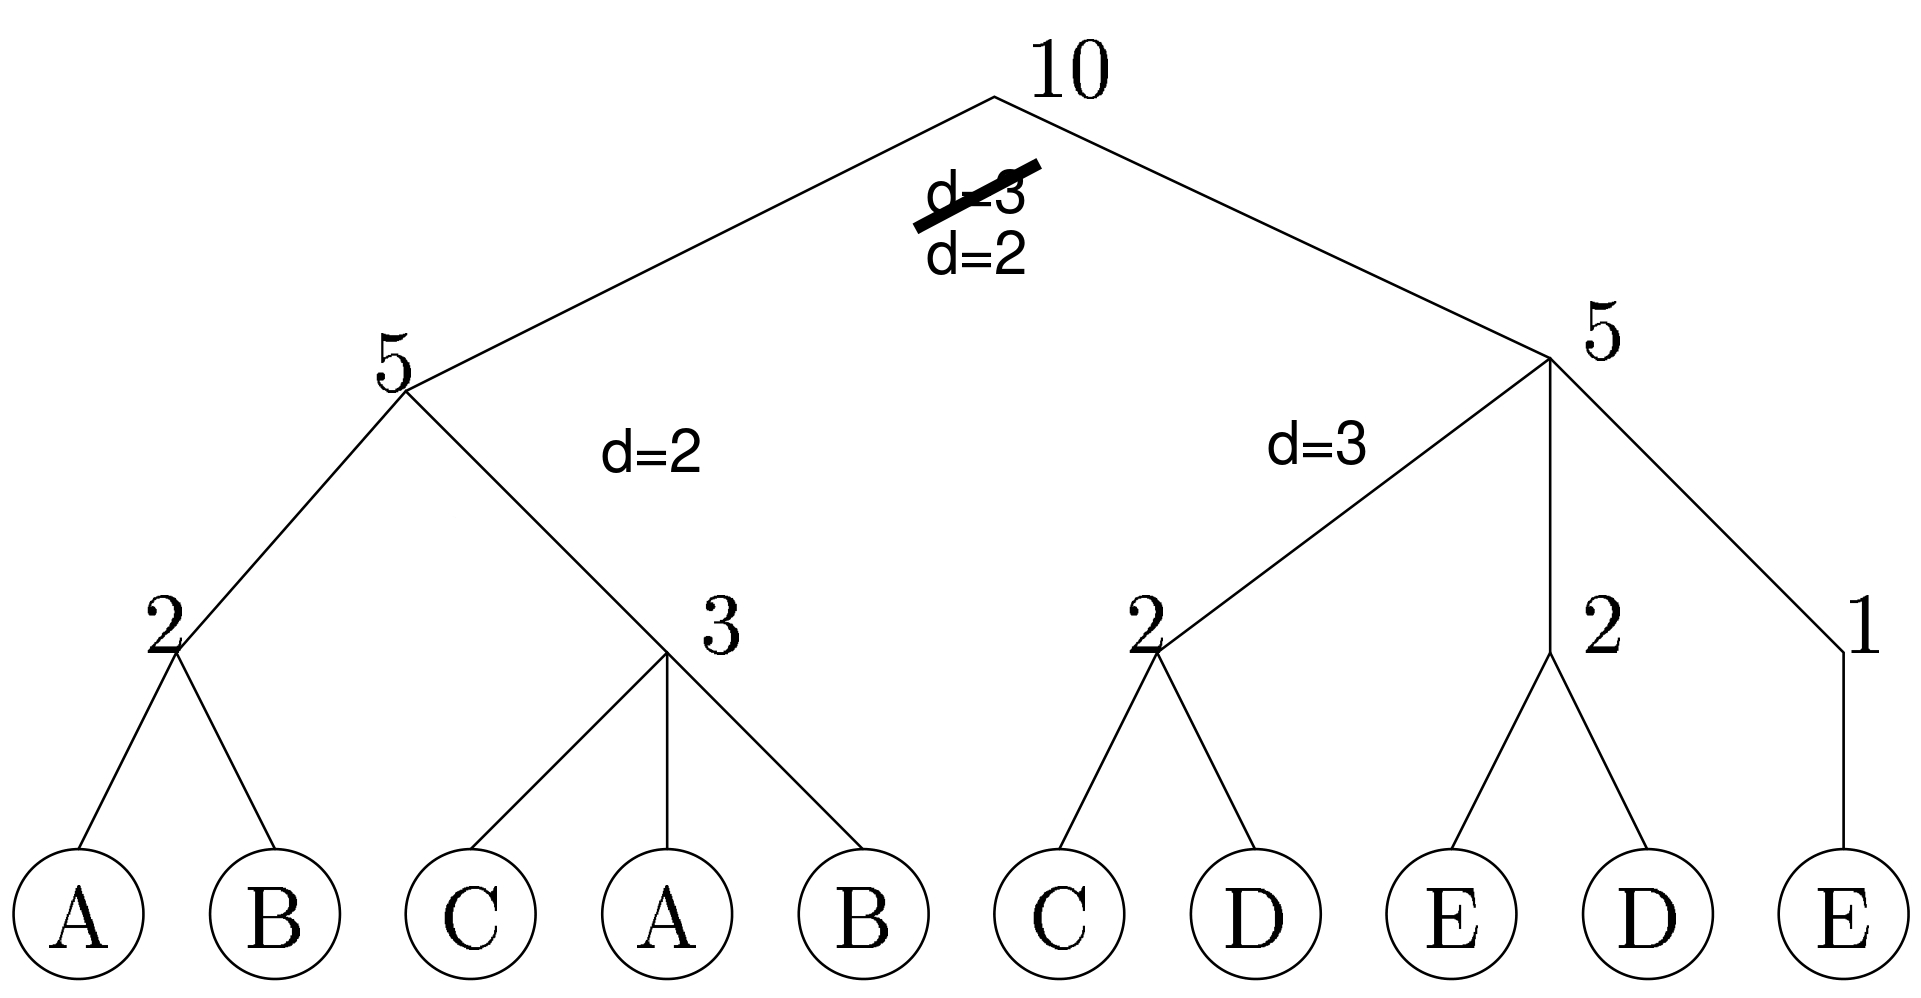
\includegraphics[scale=0.17]{creacion6.jpg}
\end{figure}}

\end{frame}



%%%%%%%%%%%%%%%%%%%%%%%%%%%%%%%%%%%%%%%%%%%%%%%%%%%%%%%%%%%%%%%%%%%%%%%%%%%%%%%%%%%%%%%%%%%%%%%%%%%%

\begin{frame}
\frametitle{Insercion}
  Insercion(i,b, T). Inserto el nodo hoja en la i-esima posicion y los nodos que le siguen son agrupados
  como se hace con  \texttt{Create}.
  Cuando la forma de agrupar las hojas se sincroniza con la agrupacion previa se finaliza, con
  la posibilidad de tener que insertar un nuevo nodo en el nivel anterior.

  Voy a tener un loop en el cual nivel por nivel, arrancando desde h-1, con h la altura del arbol.
  En cada uno arranco por el nodo que esta en el camino que va de la raiz al nodo insertado.

  Reorganizo los hijos de este nodo de la misma forma que con \texttt{Create}, y voy creando
  nodos vecinos a continuacion en caso de necesitarlo.
  Cuando llego a una sincronizacion con la estructura original freno y paso al nivel anterior, donde
  se tiene que repetir el paso esta vez contemplando los nuevos nodos creados.

  En casos donde estoy parado en el ultimo nodo de un nivel puede terminarse antes ya que se sincroniza
  con la estrucutra anterior.

   Al finalizar computno nuevamente la informacion de los tamaños de los nodos modificados.
\end{frame}

%%%%%%%%%%%%%%%%%%%%%%%%%%%%%%%%%%%%%%%%%%%%%%%%%%%%%%%%%%%%%%%%%%%%%%%%%%%%%%%%%%%%%%%%%%%%%%%%%%%%

\section{}
\begin{frame}
\frametitle{}


\end{frame}

%%%%%%%%%%%%%%%%%%%%%%%%%%%%%%%%%%%%%%%%%%%%%%%%%%%%%%%%%%%%%%%%%%%%%%%%%%%%%%%%%%%%%%%%%%%%%%%%%%%%

\section{}
\begin{frame}
\frametitle{Borrado}

  Tiempo: O(logn)

\end{frame}

%%%%%%%%%%%%%%%%%%%%%%%%%%%%%%%%%%%%%%%%%%%%%%%%%%%%%%%%%%%%%%%%%%%%%%%%%%%%%%%%%%%%%%%%%%%%%%%%%%%%

\section{}
\begin{frame}
\frametitle{}


\end{frame}

%%%%%%%%%%%%%%%%%%%%%%%%%%%%%%%%%%%%%%%%%%%%%%%%%%%%%%%%%%%%%%%%%%%%%%%%%%%%%%%%%%%%%%%%%%%%%%%%%%%%

\section{}
\begin{frame}
\frametitle{}


\end{frame}

%%%%%%%%%%%%%%%%%%%%%%%%%%%%%%%%%%%%%%%%%%%%%%%%%%%%%%%%%%%%%%%%%%%%%%%%%%%%%%%%%%%%%%%%%%%%%%%%%%%%

\section{}
\begin{frame}
\frametitle{}


\end{frame}

%%%%%%%%%%%%%%%%%%%%%%%%%%%%%%%%%%%%%%%%%%%%%%%%%%%%%%%%%%%%%%%%%%%%%%%%%%%%%%%%%%%%%%%%%%%%%%%%%%%%

\section{}
\begin{frame}
\frametitle{}


\end{frame}

%%%%%%%%%%%%%%%%%%%%%%%%%%%%%%%%%%%%%%%%%%%%%%%%%%%%%%%%%%%%%%%%%%%%%%%%%%%%%%%%%%%%%%%%%%%%%%%%%%%%

\section{}
\begin{frame}
\frametitle{}


\end{frame}

%%%%%%%%%%%%%%%%%%%%%%%%%%%%%%%%%%%%%%%%%%%%%%%%%%%%%%%%%%%%%%%%%%%%%%%%%%%%%%%%%%%%%%%%%%%%%%%%%%%%

\section{}
\begin{frame}
\frametitle{}


\end{frame}

%%%%%%%%%%%%%%%%%%%%%%%%%%%%%%%%%%%%%%%%%%%%%%%%%%%%%%%%%%%%%%%%%%%%%%%%%%%%%%%%%%%%%%%%%%%%%%%%%%%%

\section{}
\begin{frame}
\frametitle{}

\huge
\centering
FIN!
\end{frame}

%%%%%%%%%%%%%%%%%%%%%%%%%%%%%%%%%%%%%%%%%%%%%%%%%%%%%%%%%%%%%%%%%%%%%%%%%%%%%%%%%%%%%%%%%%%%%%%%%%%%

%%%%%%%%%%%%%%%%%%%%%%%%%%%%%%%%%%%%%%%%%%%%%%%%%%%%%%%%%%%%%%%%%%%%%%%%%%%%%%%%%%%%%%%%%%%%%%%%%%%%

\begin{frame}
\frametitle{Insercion}
  \begin{enumerate}
    \item  Busco la i posicion con la info de los nodos e inserto
  ahi el nodo en i+1.
  \item Voy nivel por nivel desde el ultimo hacia arriba.
  En cada uno tengo dos casos.
  \begin{itemize}
    \item Ultimo nodo:
      \begin{itemize}
        \item as
      \end{itemize}
    \item En caso contrario, inicializo una variable w=1 y repito los siguientes pasos hasta que w=0.
      \begin{itemize}
        \item
      \end{itemize}
  \end{itemize}
\item Si l$\leq$0,
\end{enumerate}
  Tiempo: O(logn)

  The way the nodes up to $u_{l+1}$ are grouped is not changed by Insert.
  The nodes after $u_{l+1}$ are grouped exactly in the same way as algorithm Create would,
  but using new coin tosses.
  This defines the topology of the nodes up to $u_l$.
  The nodes after $u_l$ are not modified.

\end{frame}

%%%%%%%%%%%%%%%%%%%%%%%%%%%%%%%%%%%%%%%%%%%%%%%%%%%%%%%%%%%%%%%%%%%%%%%%%%%%%%%%%%%%%%%%%%%%%%%%%%%%

\end{document}

